\section{度量熵}

对于次高斯

%ε网、ε包、ε覆盖、均匀离散集、相对密集集和德尔尼集(以鲍里斯·德尔尼命名)是几个紧密相关的定义,用于描述点集的良好分布,这些集合的包络半径和覆盖半径衡量了它们的分布情况。
%这些集合在编码、近似算法等理论中有着应用. 

在度量空间理论中, $\delta$-网,  $\delta$-覆盖, $\delta$-填装是几个紧密相关的定义,可以用于描述点集的良好分布. 

集合$\bT \subseteq \cX$关于度量$\rho$的一个$\delta$-覆盖是指


不要相聚太远、也不要过于拥挤——稀疏有致的点

\begin{figure}[H]
	\centering 
	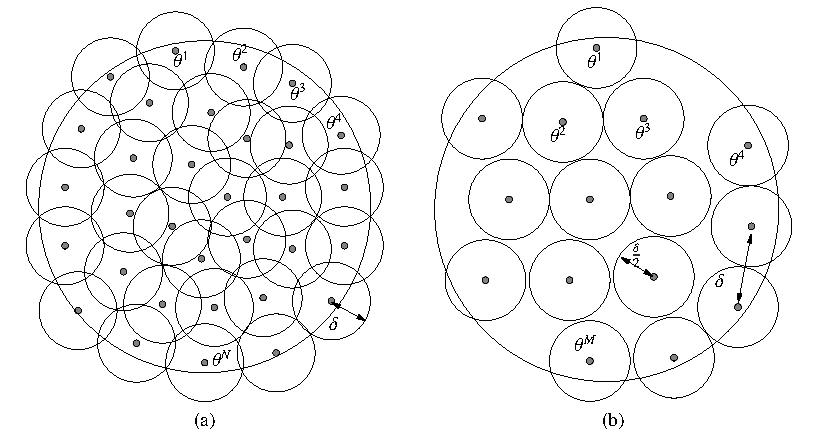
\includegraphics[width=.95\textwidth]{figure/covering-packing.pdf}
\end{figure}


\begin{figure}[H]
	\centering 
	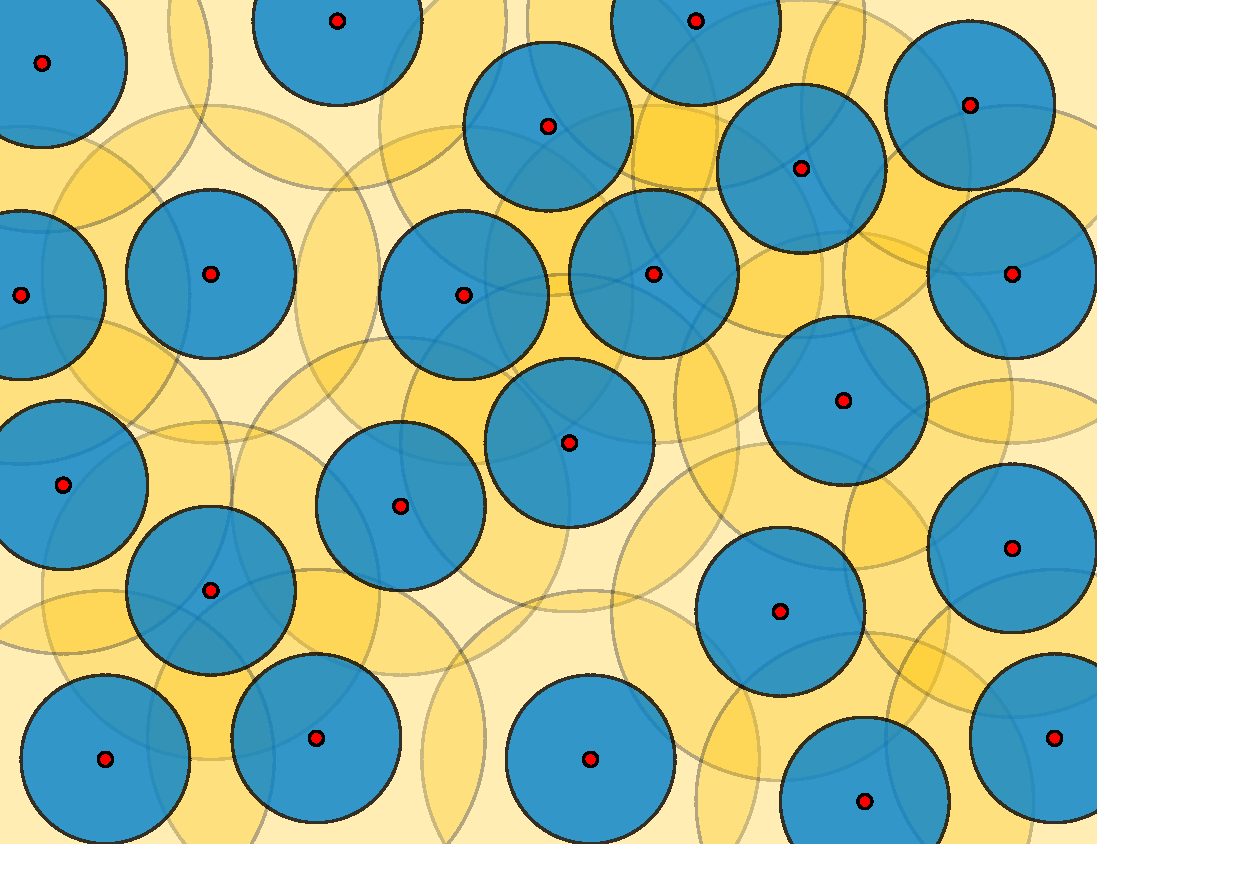
\includegraphics[width=.5\textwidth]{figure/Metric_epsilon-net.pdf}
\end{figure}







